\hypertarget{group__STM32F3xx__System__Private__Functions}{}\section{S\+T\+M32\+F3xx\+\_\+\+System\+\_\+\+Private\+\_\+\+Functions}
\label{group__STM32F3xx__System__Private__Functions}\index{S\+T\+M32\+F3xx\+\_\+\+System\+\_\+\+Private\+\_\+\+Functions@{S\+T\+M32\+F3xx\+\_\+\+System\+\_\+\+Private\+\_\+\+Functions}}
Collaboration diagram for S\+T\+M32\+F3xx\+\_\+\+System\+\_\+\+Private\+\_\+\+Functions\+:\nopagebreak
\begin{figure}[H]
\begin{center}
\leavevmode
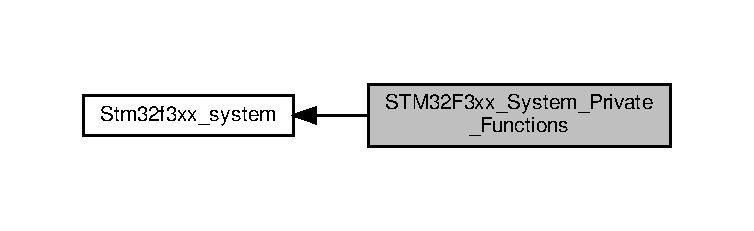
\includegraphics[width=350pt]{group__STM32F3xx__System__Private__Functions}
\end{center}
\end{figure}


\subsection{Detailed Description}


\subsection{Function Documentation}
\mbox{\Hypertarget{group__STM32F3xx__System__Private__Functions_ga19a0c3ef7421e9045e62d7df7f1120a9}\label{group__STM32F3xx__System__Private__Functions_ga19a0c3ef7421e9045e62d7df7f1120a9}} 
\index{S\+T\+M32\+F3xx\+\_\+\+System\+\_\+\+Private\+\_\+\+Functions@{S\+T\+M32\+F3xx\+\_\+\+System\+\_\+\+Private\+\_\+\+Functions}!System\+Core\+Clock\+Update@{System\+Core\+Clock\+Update}}
\index{System\+Core\+Clock\+Update@{System\+Core\+Clock\+Update}!S\+T\+M32\+F3xx\+\_\+\+System\+\_\+\+Private\+\_\+\+Functions@{S\+T\+M32\+F3xx\+\_\+\+System\+\_\+\+Private\+\_\+\+Functions}}
\subsubsection{\texorpdfstring{System\+Core\+Clock\+Update()}{SystemCoreClockUpdate()}}
{\footnotesize\ttfamily void System\+Core\+Clock\+Update (\begin{DoxyParamCaption}\item[{void}]{ }\end{DoxyParamCaption})}



Update System\+Core\+Clock variable according to Clock Register Values. The System\+Core\+Clock variable contains the core clock (H\+C\+LK), it can be used by the user application to setup the Sys\+Tick timer or configure other parameters. 

\begin{DoxyNote}{Note}
Each time the core clock (H\+C\+LK) changes, this function must be called to update System\+Core\+Clock variable value. Otherwise, any configuration based on this variable will be incorrect.

-\/ The system frequency computed by this function is not the real frequency in the chip. It is calculated based on the predefined constant and the selected clock source\+:
\end{DoxyNote}

\begin{DoxyItemize}
\item If S\+Y\+S\+C\+LK source is H\+SI, System\+Core\+Clock will contain the H\+S\+I\+\_\+\+V\+A\+L\+U\+E($\ast$)
\item If S\+Y\+S\+C\+LK source is H\+SE, System\+Core\+Clock will contain the H\+S\+E\+\_\+\+V\+A\+L\+U\+E($\ast$$\ast$)
\item If S\+Y\+S\+C\+LK source is P\+LL, System\+Core\+Clock will contain the H\+S\+E\+\_\+\+V\+A\+L\+U\+E($\ast$$\ast$) or H\+S\+I\+\_\+\+V\+A\+L\+U\+E($\ast$) multiplied/divided by the P\+LL factors.
\end{DoxyItemize}

($\ast$) H\+S\+I\+\_\+\+V\+A\+L\+UE is a constant defined in stm32f3xx\+\_\+hal.\+h file (default value 8 M\+Hz) but the real value may vary depending on the variations in voltage and temperature.

($\ast$$\ast$) H\+S\+E\+\_\+\+V\+A\+L\+UE is a constant defined in stm32f3xx\+\_\+hal.\+h file (default value 8 M\+Hz), user has to ensure that H\+S\+E\+\_\+\+V\+A\+L\+UE is same as the real frequency of the crystal used. Otherwise, this function may have wrong result.


\begin{DoxyItemize}
\item The result of this function could be not correct when using fractional value for H\+SE crystal.
\end{DoxyItemize}


\begin{DoxyParams}{Parameters}
{\em None} & \\
\hline
\end{DoxyParams}

\begin{DoxyRetVals}{Return values}
{\em None} & \\
\hline
\end{DoxyRetVals}
\mbox{\Hypertarget{group__STM32F3xx__System__Private__Functions_gaf019145746f780cda3053023bd6c1819}\label{group__STM32F3xx__System__Private__Functions_gaf019145746f780cda3053023bd6c1819}} 
\index{S\+T\+M32\+F3xx\+\_\+\+System\+\_\+\+Private\+\_\+\+Functions@{S\+T\+M32\+F3xx\+\_\+\+System\+\_\+\+Private\+\_\+\+Functions}!System\+Init@{System\+Init}}
\index{System\+Init@{System\+Init}!S\+T\+M32\+F3xx\+\_\+\+System\+\_\+\+Private\+\_\+\+Functions@{S\+T\+M32\+F3xx\+\_\+\+System\+\_\+\+Private\+\_\+\+Functions}}
\subsubsection{\texorpdfstring{System\+Init()}{SystemInit()}}
{\footnotesize\ttfamily void System\+Init (\begin{DoxyParamCaption}\item[{void}]{ }\end{DoxyParamCaption})}



Setup the microcontroller system Initialize the F\+PU setting, vector table location and the P\+LL configuration is reset. 


\begin{DoxyParams}{Parameters}
{\em None} & \\
\hline
\end{DoxyParams}

\begin{DoxyRetVals}{Return values}
{\em None} & \\
\hline
\end{DoxyRetVals}
